\pagestyle{fancy}
\fancyhf{}
\fancyhead[OL]{\rightmark}
\cfoot{\thepage}

\chapter{Introduzione}
\label{introduzione}

\begin{chapquote}{Douglas Adams, \textit{Guida galattica per gli autostoppisti}}
"È importante e risaputo che le cose non sempre sono ciò che appaiono. Per esempio sul pianeta Terra gli uomini hanno sempre ritenuto di essere più intelligenti dei delfini. Sostenevano infatti che mentre loro avevano inventato un sacco di cose, come la ruota, New York, le guerre, ecc., i delfini non avevano fatto altro che sguazzare nell'acqua divertendosi. Al contrario invece, i delfini sapevano da tempo dell'imminente distruzione della Terra e avevano tentato più volte di avvertire l'umanità dell'incombente pericolo; ma i loro messaggi erano stati fraintesi e interpretati come divertenti tentativi di dare calci a palle da football o di fischiare per avere bocconcini prelibati. Così alla fine i delfini rinunciarono e se ne andarono dalla Terra coi propri mezzi, poco prima che arrivassero i vogon."
\end{chapquote}
\vspace{5mm}

Il presente lavoro di tesi ha come oggetto lo sviluppo di un modello di classificazione in grado di discriminare il contenuto informativo di un'immagine, verificando se essa raffiguri o meno una pinna dorsale di un delfino. Questo modello si propone come un'alternativa migliore (in quanto a prestazioni raggiunte) rispetto al modello nativo presente in \textit{CropFin v1}, una routine che effettua il rilevamento e l'estrazione di eventuali pinne di delfini presenti in un'immagine. La routine \textit{CropFin v1} è frutto di un precedente lavoro di tesi triennale \cite{gianvito}, di cui questo elaborato vuole essere una naturale prosecuzione.
Il miglioramento delle prestazioni della classificazione di CropFin v1 si innesta in un più ampio contesto di lavoro: quello della foto-identificazione dei cetacei (par. \ref{fotoidentificazione}).\\

Il presente lavoro di tesi è stato sviluppato nel corso di un'attività di tirocinio presso l'Istituto \textit{STIIMA}\footnote{Sistemi e Tecnologie Industriali Intelligenti per il Manifatturiero Avanzato, \url{stiima.cnr.it/it}} del Consiglio Nazionale delle Ricerche di Bari, sotto la supervisione del Dott. Vito Renò.
In particolare, la proposta di tesi è nata nell'ambito di una collaborazione dell'istituto con le associazioni di ricerca scientifica \textit{Jonian Dolphin Conservation}\footnote{\url{joniandolphin.it}}, finalizzata allo studio dei cetacei nel Golfo di Taranto (Mar Ionio Settentrionale), e \textit{Nova Atlantis Foundation}\footnote{\url{nova-atlantis.org}}, finalizzata allo studio dei cetacei nell'area delle isole Azzorre (Oceano Pacifico).

\begin{figure}[h!]
  \begin{minipage}[b]{0.45\textwidth}
  \centering
    
\includegraphics[width=0.8\textwidth]{jonian}
    \caption{Logo della Jonian Dolphin Conservation}
    \label{fig:jdc}
  \end{minipage}
  \hfill
  \begin{minipage}[b]{0.45\textwidth}
  \centering
    
\includegraphics[width=0.8\textwidth]{nova}
    \caption{Logo della Nova Atlantis Foundation}
    \label{fig:naf}
  \end{minipage}
\end{figure}

Il principale risultato della collaborazione con \textit{Jonian Dolphin Conservation}, presentato in \cite{maglietta}, è stata la creazione di una piattaforma innovativa per lo studio dei delfini della specie \textit{Grampus griseus} nel Golfo di Taranto, chiamati comunemente delfini di Risso o grampi. La piattaforma\footnote{\url{http://dolfin.ba.issia.cnr.it}} contiene una serie di dati di avvistamento e foto georeferenziate collezionate tra il 2013 ed il 2016. È stato inoltre introdotto un \textit{tool} innovativo per la foto-identificazione automatica degli esemplari, creando i principali presupposti per le idee alla base del presente lavoro di tesi. Questo aspetto è chiarito con maggior dettaglio nel paragrafo seguente \ref{fotoidentificazione}.

Nei paragrafi seguenti si approfondiscono i motivi dell'interesse scientifico verso i cetacei, in seguito si fornisce una descrizione più dettagliata del problema affrontato ed infine si espongono lavori simili all’interno del panorama scientifico internazionale.


\section{Interessi scientifici}
\label{contesto}
Il monitoraggio della distribuzione dei cetacei e della sua mutazione nel tempo costituisce un elemento determinante per la comprensione dell'alterazione degli ecosistemi marini. È noto, infatti, che lo stato di salute di ecosistemi con catene alimentari lunghe, come quello marino, si rifletta nella presenza e nell'abbondanza dei predatori dei livelli trofici superiori; tra questi figurano proprio i delfini.

Studiare i delfini significa, quindi, conoscere indirettamente lo stato di salute dell'ecosistema marino in cui sono inseriti. Ciò risulta di particolare rilevanza per il Golfo di Taranto, poiché soggetto da anni ad un grave livello di inquinamento ambientale a causa degli insediamenti industriali presenti nella zona. Il monitoraggio degli ecosistemi marini è, in ogni caso, considerato necessario secondo alcune recenti direttive emesse dall'Unione Europea\footnote{EU Marine Strategy Framework Directive (\url{https://ec.europa.eu/environment/marine/eu-coast-and-marine-policy/marine-strategy-framework-directive/index_en.htm}), Maritime Spatial Planning Directive (\url{https://ec.europa.eu/maritimeaffairs/policy/maritime_spatial_planning_en})}.\\

Quello marino è solo un esempio dei tanti ecosistemi costantemente minacciati dall'impatto delle attività antropiche; al giorno d'oggi si stima che alterazioni irreversibili siano già in atto. Il tema dei cambiamenti climatici ha assunto, non a caso, importanza centrale nei dibattiti internazionali recenti e causa continue mobilitazioni di carattere globale.


\section{Foto-identificazione automatica del \\\textit{Grampus griseus}}
\label{fotoidentificazione}
La foto-identificazione è una tecnica di studio non invasiva basata sull'ipotesi generale che ciascun individuo può essere identificato in maniera univoca all'interno della popolazione grazie a specifiche caratteristiche fisiche distintive.

La foto-identificazione dei singoli individui nell'ambito dello studio dei cetacei è ritenuta di particolare utilità poichè consente di ottenere conoscenze più dettagliate sulle relazioni sociali all'interno della popolazione e sull'ambiente marino in cui gli esemplari vivono, senza arrecare disturbo agli stessi.

I delfini della specie \textit{Grampus griseus} presentano numerose peculiarità che li rendono differenti dalle altre specie spesso associate all'immaginario comune, una su tutte quella del \textit{Tursiops truncatus} (tursiope). Inoltre, presentano un tratto distintivo, descritto in dettaglio più avanti, che li rende particolarmente adatti ad essere studiati con la tecnica della foto-identificazione automatica. La fig. \ref{fig:delfini} mette a confronto le specie citate.

\begin{figure}[h!]
	\centering
	\begin{subfigure}[b]{0.45\textwidth}
	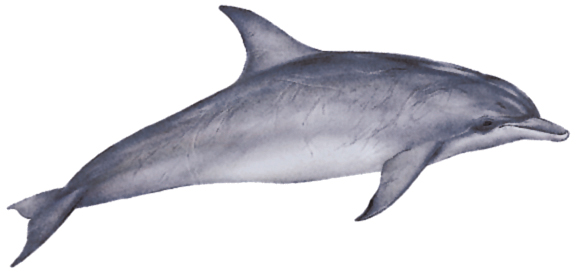
\includegraphics[width=\linewidth]{tusiops}
	\caption{}
	\end{subfigure}
	\begin{subfigure}[b]{0.45\textwidth}
	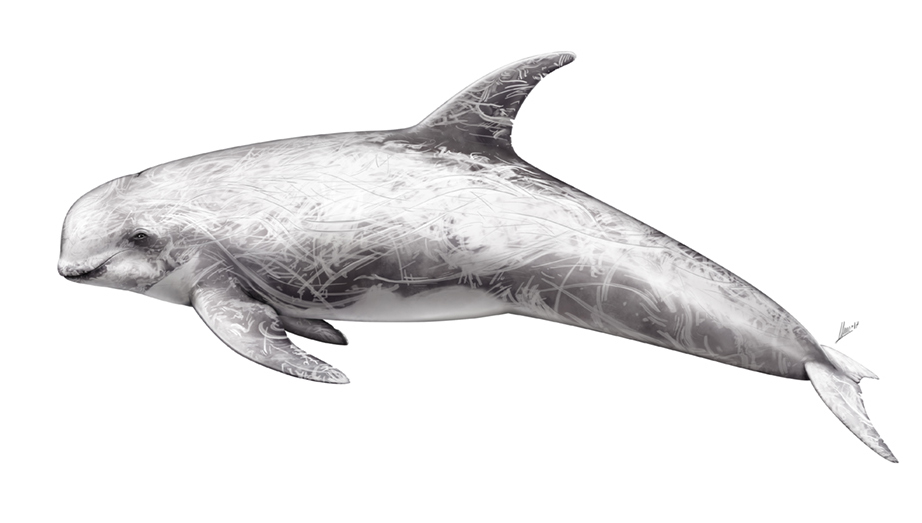
\includegraphics[width=\linewidth]{grampus}
	\caption{}
	\end{subfigure}
	\caption{Illustrazione delle specie a confronto: (a) \textit{Tusiops truncatus} (tursiope) (crediti: \protect\url{animalbase.uni-goettingen.de}), (b) \textit{Grampus griseus} (grampo) (crediti: \protect\url{associaciocetacea.org}).}
	\label{fig:delfini}
\end{figure}

La specie \textit{Grampus griseus}, ai cui esemplari ci si riferisce nel seguito semplicemente come grampi, è distribuita dai tropici fino alle regioni temperate in entrambi gli emisferi terrestri. Un individuo in età adulta può avere una lunghezza compresa tra 2,5 e 4 metri ed un peso di 500-600 kg. A differenza del tursiope, il capo si presenta senza rostro sul davanti e con un largo sfiatatoio nella parte superiore. La pinna dorsale, posta circa a metà del corpo, è particolarmente alta ed appuntita e presenta una curvatura piuttosto accentuata.

Come si può ben notare nella fig.\ref{fig:grampo}, l'intero corpo dei grampi, pinna dorsale inclusa, è generalmente ricoperto da una quantità notevole di graffi di tonalità molto chiara. La comparsa di questi segni avviene in modo graduale nel corso della vita dell'animale: alla nascita, infatti, il colore del corpo è scuro e uniforme. Si sostiene che essi siano provocati dalle interazioni sia di carattere alimentare con le prede sia di carattere sociale con gli altri individui. Gli esemplari più anziani ne vantano così tanti da risultare praticamente bianchi.

\begin{figure}[h!]
	\centering
	\includegraphics[width=0.8\linewidth]{gr}
	\caption{Esemplare di grampo nel Golfo di Taranto (crediti: Emanuele Seller \cite{emanuele})}
	\label{fig:grampo}
\end{figure}

La peculiarità appena descritta è proprio il tratto fisico distintivo che consente di applicare la tecnica di foto-identificazione agli esemplari di grampo. I soli graffi presenti sulla pinna dorsale sono, infatti, paragonabili alle impronte digitali dell'uomo: ogni individuo presenta un \textit{pattern} di segni unico che lo contraddistingue all'interno della popolazione.

\begin{figure}[h!]
	\centering
	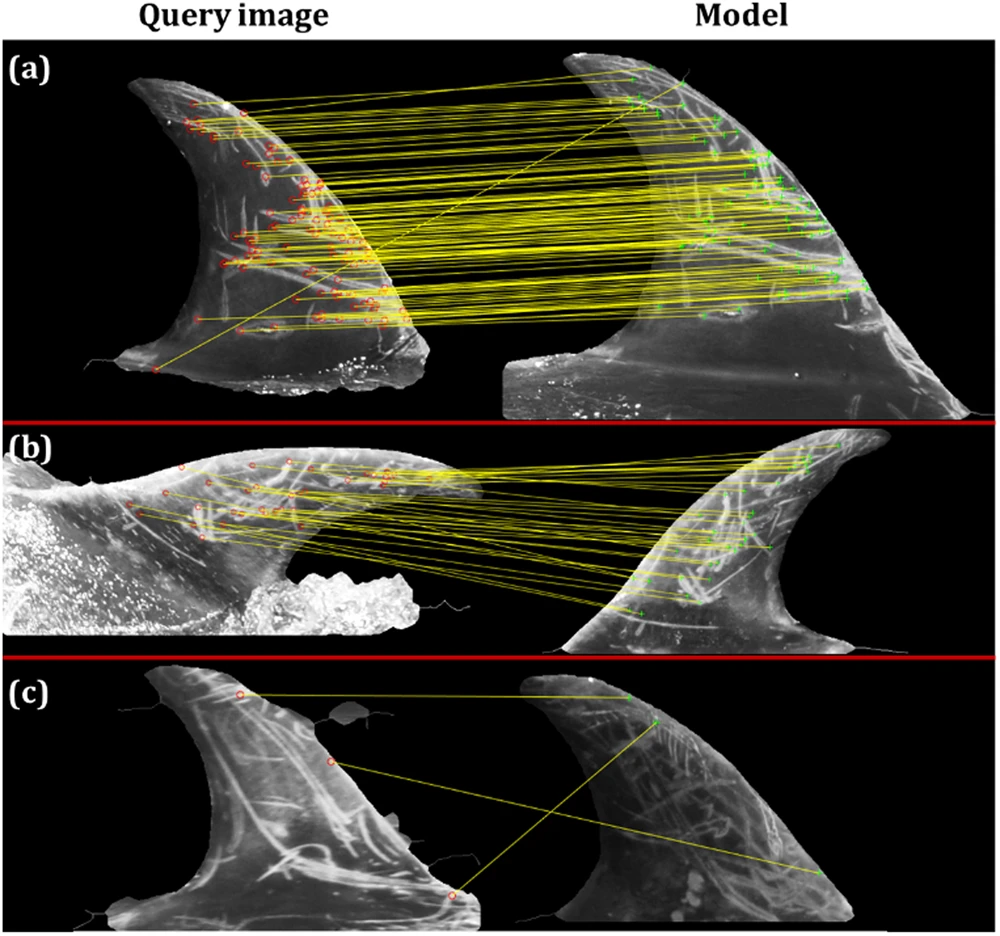
\includegraphics[width=0.75\linewidth]{spir2}
	\caption{Esempio di output dell'algoritmo \textit{SPIR}: nell'ordine predizione corretta, predizione corretta di una pinna ruotata, predizione non corretta. Immagine tratta da \cite{maglietta}.}
	\label{fig:dalpaper}
\end{figure}

Nell'ambito dello studio \cite{maglietta} già citato in precedenza, si è fatto uso di questa tecnica per stimare, a partire dalla grande quantità di immagini raccolta nel corso di campagne di avvistamento effettuate negli ultimi anni dall'associazione \textit{Jonian Dolphin Conservation}, la distribuzione, l'abbondanza e le relazioni sociali di una popolazione di grampi stanziata nel Golfo di Taranto.
Il risultato ottenuto si rivela di grande importanza poichè sopperisce ad una quasi totale assenza di dati: la IUCN \textit{Red List of Threatened Species} ha considerato (fino a pochi anni fa) i grampi come specie “data deficient” nella zona del Mar Mediterraneo\footnote{\url{https://www.iucnredlist.org/species/16378423/16378453}}.\\

Come accennato nel paragrafo precedente, un altro risultato importante è stato l'introduzione di un tool innovativo per la foto-identificazione automatica, denominato \textit{SPIR} (\textit{Smart Photo-Identification of Risso's dolphins}). Esso permette l’identificazione degli esemplari di grampo senza alcun intervento da parte dell’utente (fig. \ref{fig:dalpaper}).

L'introduzione di \textit{SPIR} costituisce il passo fondamentale per la concretizzazione della possibilità di impiegare la tecnica di foto-identificazione nell'ambito di nuovi studi su larga scala, superando parte delle criticità, temporali e non solo, legate all'analisi di grandi quantità di immagini (\textit{big data}) in maniera manuale.\\

La completa automatizzazione della procedura resta, tuttavia, vincolata al superamento di un'ulteriore criticità: la \textbf{necessità di ritagliare le pinne dorsali a partire dalle immagini iniziali} (fig. \ref{fig:ritagliopinna}).

\begin{figure}[h!]
	\centering
	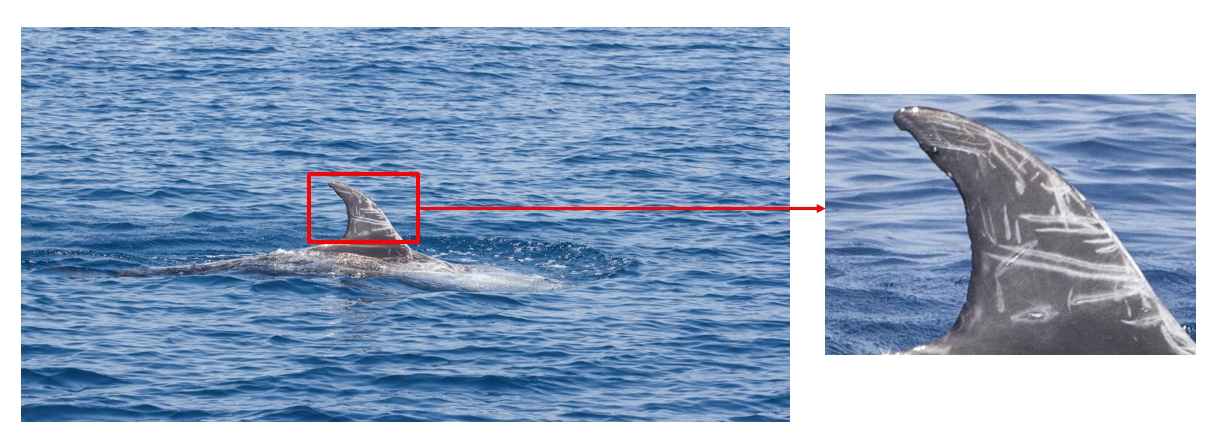
\includegraphics[width=0.9\linewidth]{ritagliopinna}
	\caption{Ritaglio di una pinna dorsale di un delfino da un'immagine.}
	\label{fig:ritagliopinna}
\end{figure}

La fase del ritaglio, se fatta manualmente, risulta infatti un collo di bottiglia all'interno della procedura di foto-identificazione automatica, essendo particolarmente dispendiosa in temrini di tempo.

L'algoritmo CropFin v1, presentato in \cite{gianvito} e basato su un precedente lavoro \cite{flavio} ha avuto l'obiettivo di automatizzare la fase di ritaglio delle pinne dorsali a partire dalla collezione delle immagini scattate in mare, consacrando in maniera definitiva la foto-identificazione automatica come la tecnica di studio non invasiva di maggiore efficienza per lo studio della specie \textit{Grampus griseus} su larga scala.\\

\section{Problema ed obiettivi}
Il presente lavoro di tesi vuole porsi come una naturale prosecuzione rispetto ai lavori \cite{gianvito} e \cite{flavio}.
Il lavoro è consistito nell'apportare un miglioramento delle prestazioni della fase di classificazione dei ritagli previsto dalla routine CropFin v1.
La principale tecnica utilizzata per apportare questo miglioramento è il \textit{transfer learning} (par. \ref{transferLearning}), il cui studio è centrale nel presente elaborato.

Il risultato del lavoro è stato la creazione di una routine CropFin migliorata rispetto alla sua versione v1, con prestazioni nettamente superiori ed in grado di rendere più fine ed efficace la discriminazione tra immagini contenenti pinne e quelle invece prive di valore informativo.\\

Tecnicamente, il problema affrontato può essere ricondotto ad una particolare classe
di problemi della computer vision nota come \textit{object detection}, finalizzata al riconoscimento
automatico di oggetti all’interno di immagini (par. \ref{objectDetection}).
Le metodologie risolutive utilizzate spaziano dall’\textit{Image Processing} (par. \ref{imDig}) al \textit{Machine
Learning} (par. \ref{machineLearning}).\\

Nel cap. \ref{teoria} vengono descritti le metodologie ed i concetti teorici utilizzati all'interno degli esperimenti svolti; il cap. \ref{esperimenti} descrive dettagliatamente gli esperimenti svolti; nel cap. \ref{conclusioni} sono esposte
considerazioni finali sulle soluzioni proposte, e vengono presentati alcuni sviluppi futuri e miglioramenti apportabili alla routine messa a punto; infine, nel cap. \ref{sorgenti} si riporta il codice sorgente Matlab scritto ed adoperato negli esperimenti.\\

Questo lavoro può essere inquadrato nell’ambito di una disciplina emergente al
confine tra ecologia e informatica, nota come \textit{ecological informatics}.
Come riporta l’omonima rivista scientifica\footnote{\textit{Ecological Informatics}, Elsevier}, essa si fonda sull’incontro tra la
grande quantità di dati intrinsecamente connessa all’ecologia e la crescente capacità
delle tecnologie dell’informazione di analizzare grandi moli di dati (\textit{big data}), talvolta complessi, con l’obiettivo di stimolare ed accelerare
l’avvento dei processi sostenibili in vista dei cambiamenti climatici e ambientali
globali.\\

\section{Lavori simili}
\label{lavorisimili}
Negli ultimi anni, molte tecniche di computer vision e machine learning, che operano sinergicamente in una nuova disciplina chiamata \textit{visual data analytics}, stanno assumendo un ruolo sempre più importante nelle strategie di monitoraggio e conservazione della fauna del nostro pianeta.

In questo contesto si inserisce il presente lavoro di tesi, che migliorando le prestazioni della fase che precede la foto-identificazione dei grampi vuole dare un contributo concreto all'importante causa della salvaguardia degli ecosistemi.

Sono molti i lavori affini a quello presentato in questo elaborato. La maggior parte di essi sono di recente pubblicazione o ancora in fase di sviluppo. In questo paragrafo se ne presentano alcuni, ritenuti particolarmente significativi anche in virtù del loro uso del \textit{transfer learning}, tecnica su cui, come detto, si incardina il presente lavoro di tesi. L'impiego profuso di tale tecnica in queste pubblicazioni ne conferma l'efficacia e ne suggerisce l'utilizzo anche per risolvere il nostro task di classificazione delle pinne.

\paragraph*{A Hybrid Approach for Tiger Re-Identification \cite{tiger}.}
Questo lavoro si inserisce nel contesto della "\textit{Amur tiger re-identification (Re-ID) challenge}", tenuto dal workshop \textit{Computer Vision for Wildlife Conservation} nell'ambito della \textit{International Conference on Computer Vision 2019}. Il suo obiettivo è la creazione di un sistema di foto-identificazione degli esemplari di tigre siberiana (\textit{Panthera tigris altaica}), reso possibile dal particolare manto striato della specie, il cui pattern è univoco per ogni individuo, e che pertanto rende la specie particolarmente adatta alla foto-identificazione.

Alcune criticità (dataset di immagini a disposizione limitato e di bassa qualità, variazioni nell'esposizione alla luce e nella posa degli esemplari e numero limitato di immagini di ciascun esemplare) rendono la foto-identificazione di questa specie un task difficile per i modelli di deep learning. Conseguentemente, si è proposto l'utilizzo sia delle tecniche e dei modelli del deep learning e sia della tradizionale tecnica di matching basata sui descrittori SIFT.

Il modello di classificazione progettato è una rete neurale convoluzionale profonda, DenseNet-121 \cite{densenet}, ri-addestrata con la tecnica del \textit{transfer learning}. Numerose operazioni di \textit{image augmentation} sono state adoperate per incrementare la dimensione e l'eterogeneità del dataset a disposizione, migliorando la capacità di generalizzazione della rete. In fig. \ref{fig:tiger} è riportato il \textit{workflow} del sistema di foto-identificazione oggetto del paper.

\begin{figure}[h!]
\centering
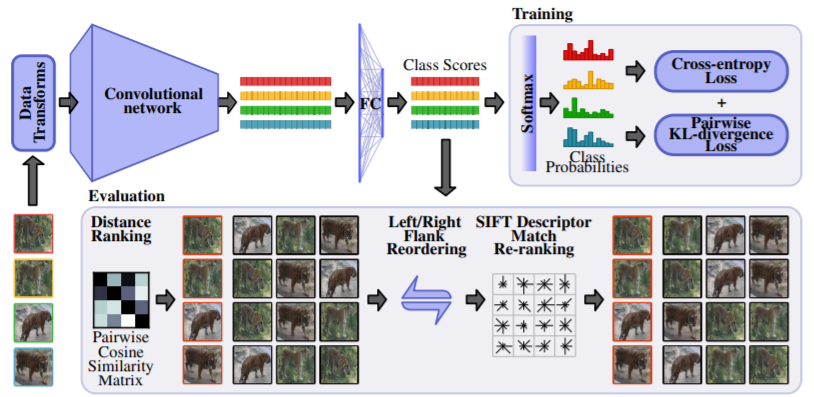
\includegraphics[width=0.9\textwidth]{tiger}
\caption{Workflow del sistema di foto-identificazione delle tigri siberiane sviluppato in \cite{tiger}. Immagine riprodotta dal paper originale.}
\label{fig:tiger}
\end{figure}


\paragraph*{Individual Minke Whale Recognition Using
Deep Learning Convolutional Neural Networks \cite{whale}.}

La balenottera minore o balenottera rostrata (Balaenoptera acutorostrata) abita un'area molto ristretta a nord della Grande Barriera Corallina australiana, durante la stagione invernale (maggio-agosto). È stato osservato che i pattern di colore di queste balene sono univoche per ogni individuo e rimangono stabili nel corso di molti anni, e sono sufficientemente complessi da rendere questa specie adatta alla foto-identificazione non equivoca degli esemplari (fig. \ref{fig:whale}).

L'identificazione degli individui di questa specie è necessaria per studiare le caratteristiche della popolazione e per monitorare l'impatto che il turismo marittimo ha su di essa. Esiste un enorme database di immagini non etichettate e non foto-identificate di balenottere minori, raccolte dalle numerose imbarcazioni turistiche che operano nell'areale della specie. Questa grande mole di dati non si presta ad una foto-identificazione manuale da parte dei biologi, e si è pertanto pensato di mettere a punto un sistema per la sua automatizzazione, ricorrendo all'uso della tecnica del \textit{transfer learning}. Una rete VGG16 pre-addestrata sul database ImageNet (par. \ref{imagenet}) è stata ri-addestrata sul dataset a disposizione, per operare una segmentazione semantica delle immagini. Per migliorare la capacità di generalizzazione della rete sono state adoperate tecniche di \textit{image augmentation}.\\

Il lavoro ha portato alla creazione della routine di foto-identificazione "\textit{Automatic Minke Whale Recognizer (AMWR)}", che raggiunge ottime prestazioni (>90\%) sui test set.

\begin{figure}[h!]
\centering
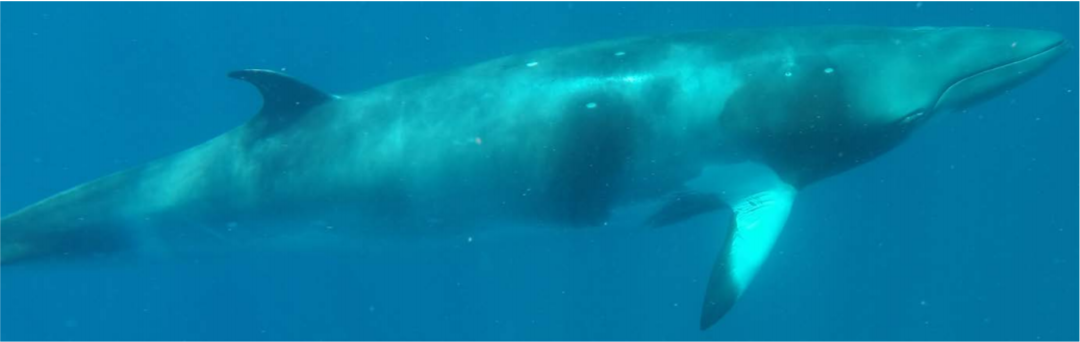
\includegraphics[width=0.85\textwidth]{whale}
\caption{Un esemplare di Balaenoptera acutorostrata. Si notino i pattern di colore della pinna e le numerose "cicatrici", caratteristiche univoche di ogni esemplare.}
\label{fig:whale}
\end{figure}

\paragraph*{Robust Re-identification of Manta Rays from Natural Markings by Learning Pose Invariant Embeddings \cite{manta}.}
In questo articolo viene presentato un nuovo metodo di foto-identificazione basato sui segni naturali univoci degli animali e robusto ad occlusioni, punti di vista e cambi di illuminazione. Il metodo è creato riadattando metodi già utilizzati per la foto-identificazione dei volti umani, ed in particolare riaddestrando la rete neurale convoluzionale FaceNet \cite{facenet} mediante la tecnica del \textit{transfer learning}. Questo nuovo metodo di foto-identificazione è generico e non specifico di una certa specie.
Il sistema è stato testato su un database di immagini di ventri di mante (Manta alfredi e Manta birostris) e su un database di pinne caudali di megattere (Megaptera novaeangliae), registrando prestazioni ottime.

\begin{figure}[h!]
\centering
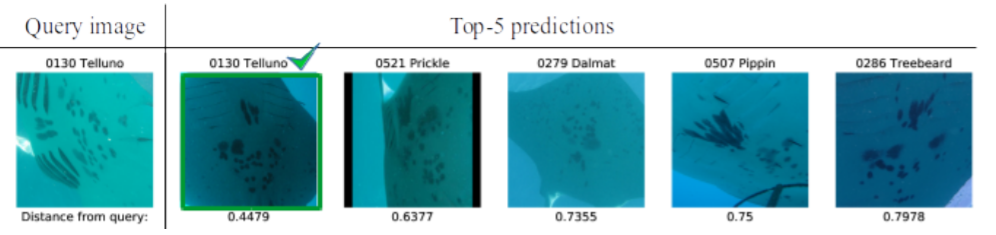
\includegraphics[width=0.9\textwidth]{manta}
\caption{Esempio di foto-identificazione di una manta avvenuta con successo. I segni scuri sul ventre della manta sono univoci per ogni esemplare, e permettono la foto-identificazione non equivoca.}
\label{fig:manta}
\end{figure}